\documentclass[a4paper,10pt]{article}
\usepackage{graphicx}
\usepackage[pdfborder={0 0 0}]{hyperref}
\title{ Student Project 2017 \\ CalTech101 Image Classification}
\author{David Schulte, Hannes Martinke, Martin Zettwitz}

\begin{document}
\maketitle

\section{Introduction}
\subsection{Problem}
The classification of arbitrary pictures is an actual very hard task for image analysts, because the machine learning methods are difficult to use with the high number of pixel features in an image.
The task of the project is to classify the \emph{CalTech 101} dataset by using different feature selection and classifing approaches. 
101 different image categories the data set contains and the aim is a valdiation accuracy of 10~\% with an 10-Fold cross validation.
\subsection{Programming Environment}
Our classification approach is implemented in C++ with the including of \emph{Opencv} and \emph{dlib}.
\emph{Opencv} and \emph{dlib} are open source libraries for computer vision and machine learning tasks. 
Out first approaches were a complete implementation in \emph{Opencv}, but because of some missing algorithm for the classification step in the library, we add the \emph{dlib} and combine both libraries in the implementation.
The workflow of our procedure is illustrated in \autoref{fig:workflow}. and consists the following 4 steps: image preprocessing, features, classifier, validation.
These steps will be explained in the next sections.

\begin{figure}[h]
\centering
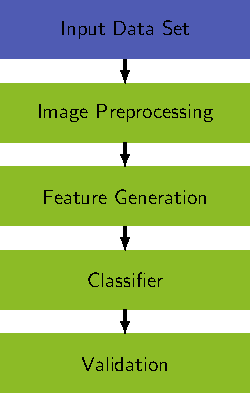
\includegraphics[scale=1]{images/Workflow.pdf}
\caption{Our Worklow for the image classification. We organized the input data sets and prepare each image for the subsequent feature generation.
This feature are integrated in the classifier and the validation is performed in the next step to evaluate the classification results.}
\label{fig:workflow}
\end{figure}

\section{Preprocessing}
Image resize to 64x64. Why?
Maybe image adding for better and more classification images

\section{Features}
\subsection{Feature Generation}
HOG features with cellsize 16. what is the solution with other cellsizes?
LBP

\subsection{Feature Reduction}
PCA? Image Resizing

\section{Classifier}
\paragraph{AdaBoost}
\paragraph{SVM}

\section{Training and Validation}
10 Fold

\section{Results}
Matrix + Conclusion 

\end{document}

